\chapter{等词与未解释函数理论命题的证明}
\label{chap:euf}

\section{输入语言}
\begin{figure}[!htbp]
  \centering
  \begin{tabular}[rcl]{rcl}
    & & $F$是未解释函数 \\
    & & $X$是整型变元 \\
    $T$ & \sep & $X$ \deli{} $F(T,$\ldots$,T)$ \\
    $Y$ & \sep{} & $T = T$ \deli{} $T \neq T$ \\
    $\Pi$ & \sep{} & $T$ \deli{} $\Pi \land \Pi$ \\
  \end{tabular}
  \caption{等词与未解释函数语言的语法}
  \label{euf:syntax}
\end{figure}
本部分接收的语言是关于变元、函数间的相等和不相等关系的合取式。目标是证明合取式的不一致性。

\section{决策过程}
\subsection{一致闭包}
一致闭包(Congruence Closure)是能解决本章形式的命题的一种效率较高的决策过程。

其基本步骤如下:
\begin{description}
\item[初始化] 对每个命题项$t_i \in T$,初始化一个集合,其初始元素为自身。
\item[合并] 对命题中的每一个相等关系$t_p = t_q$,若$t_p$和$t_q$在不同集合$S_p$和$S_q$,则合并$S_p$和$S_q$为$S_{pq}$。
\item[闭包] 反复对命题中出现的所有的相同的函数对$(f(x),f(y))$,检查$x$和$y$是否在同一集合。若在,合并$f(x)$和$f(y)$所在的集合。
\item[判断] 对不相等关系中的每一对$(x, y)$,检查$x$和$y$是否在同一集合。若在,则产生矛盾,得到不一致证明。
\end{description}

\subsection{实现}
上述算法的高效实现依赖于一个专门为上述操作设计的数据结构——并查集(Find-Union Set或Disjoint Set)。

并查集是多个树形结构组成的森林。每个树结点有一个域,指向其父结点(根结点可规定指向自身)。两个结点所代表的元素在同一个集合中,当且仅当两个结点拥有相同的根。

并查集的基本操作如下:
\begin{description}
  \item[初始化] 每个元素都指向自身。
  \item[合并] 查找两个元素的根,然后使其中一个根指向另一个。
  \item[查找] 若两个元素的根相同,则返回真,否则为假。
\end{description}

并查集还有一些优化,如按秩合并、路径压缩等。在这些优化下,其基本操作的时间复杂度约为常数。

用并查集实现一致闭包算法如图\ref{euf:set}所示。
\begin{figure}[!htbp]
  \centering
  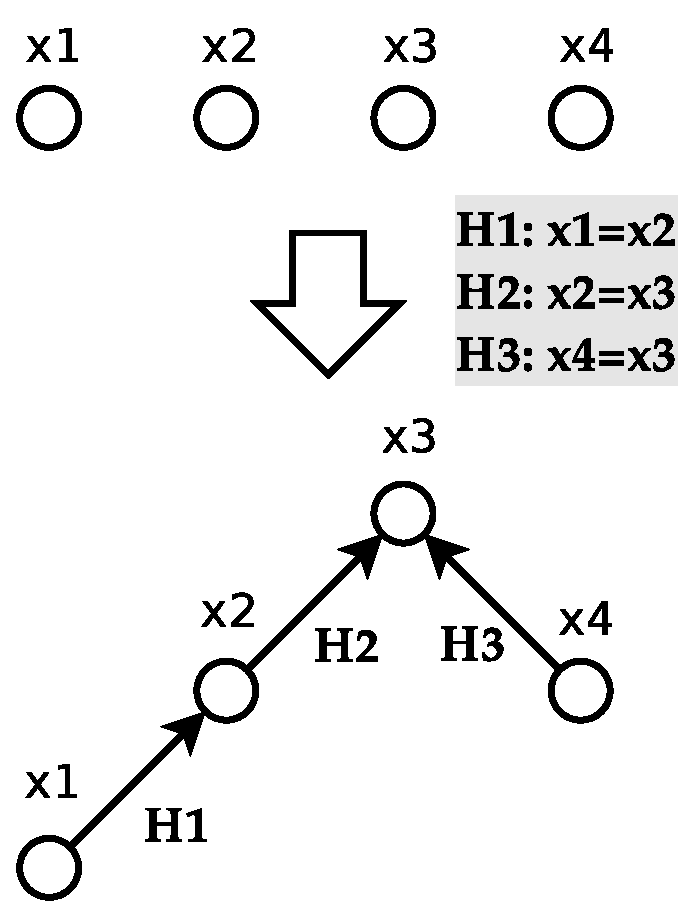
\includegraphics[width=0.35\textwidth]{euf.eps}
  \caption{并查集实现的一致闭包算法}
  \label{euf:set}
\end{figure}

\subsection{证明项的构造}
Coq中用于证明相等关系的定理有三条:
\begin{verbatim}
Lemma refl_equal : forall (A : Type) (x : A), x = x.
Lemma sym_eq : forall (A : Type) (x y : A), x = y -> y = x.
Lemma trans_eq : forall (A : Type) (x y z : A), x = y -> y = z -> x = z.
\end{verbatim}
分别对应等词的自反、对称、传递性质。

观察图\ref{euf:set},可见并查集的每一条边对应了一个相等关系。因此可以构造如下算法生成证明项(以证明$x_1=x_4$为例):
\begin{enumerate}
  \item 依传递律生成$x_1=x_3$的证明项;
  \item 依传递律生成$x_4=x_3$的证明项,再依对称律生成$x_3=x_4$的证明项;
  \item 由前两项依传递律生成$x_1=x_4$的证明项。
\end{enumerate}

以上解决了生成证明项的总体框架问题,尚需每条边所代表的相等关系的证明项。为此,我们把并查集树结点的存储由单独的父结点指针\texttt{parent}扩充为二元组\texttt{(parent, proof)},分别表示父结点指针和对应的边的证明项。

扩展后的并查集的操作算法如下:
\begin{description}
  \item[初始化] 每个元素指向自身,元素$x$的证明项为\texttt{(refl\_equal x)}。
  \item[合并] 设合并的元素对为\texttt{(u, v)},相等的证明为\texttt{H},如图\ref{euf:union}。
    \begin{enumerate}
      \item 查找\texttt{u}的根为\texttt{p},使用\texttt{trans\_eq}连接各个边的证明为\texttt{H1};
      \item 查找\texttt{v}的根为\texttt{q},使用\texttt{trans\_eq}连接各个边的证明为\texttt{H2};
      \item 令\texttt{p}的父结点为\texttt{q},附加的证明为
        \texttt{(trans\_eq (trans\_eq (sym\_eq H1) H) H2)}。
    \end{enumerate}
  \item[查找] 设查找的元素对为\texttt{(u, v)},如图\ref{euf:find}。
    \begin{enumerate}
      \item 查找\texttt{u}的根为\texttt{p},使用\texttt{trans\_eq}连接各个边的证明为\texttt{H1};
      \item 查找\texttt{v}的根为\texttt{q},使用\texttt{trans\_eq}连接各个边的证明为\texttt{H2};
      \item 若\texttt{p}和\texttt{q}不等,返回假;否则,返回真,附加的证明\texttt{(trans\_eq H1 (sym\_eq H2))}。
    \end{enumerate}

\begin{figure}[!h]
\centering
\subfigure[合并]{
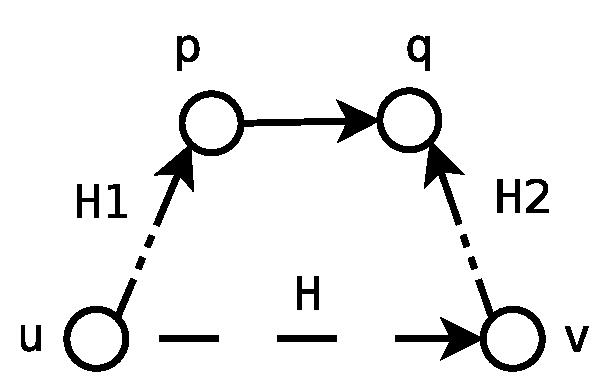
\includegraphics[width=0.32\textwidth]{euf-union.eps}\label{euf:union}}
\subfigure[查找]{
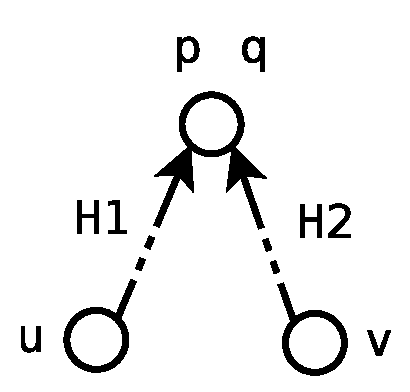
\includegraphics[width=0.22\textwidth]{euf-find.eps}\label{euf:find}}
\caption{带证明项的并查集}

\end{figure}
\end{description}


